\chapter{Root Locus}

Root locus method is another approach for control design apart from the algebriac approach used in pole placement method as described in section \ref{Sec_PolePlacement}. A polee placement technique is a simple algebriac technique which is based on algebriac manipulation of control gains in order to place the poles of the system at the locations so as to achieve certian requested property of the control system. However, pole placement technique is a rather simple technique which can be used rather fairly with canonical systems as with such system the algebriac terms relating to the control gains are very much clear. For noncanonical higher order systems this process would be much difficult to see the effect gains on all poles. For such rather complex system another technique is used called as \textbf{\textit{Root Locus Method}} for controller design.

\textbf{\textit{Root Locus}} is a graphical tool that shows how the locations of the poles of a closed-loop TF move as a parameter (like a control gain) is varied as shown in figure \ref{RootLocus_Def}.
\begin{figure}[h!]
	\centering
	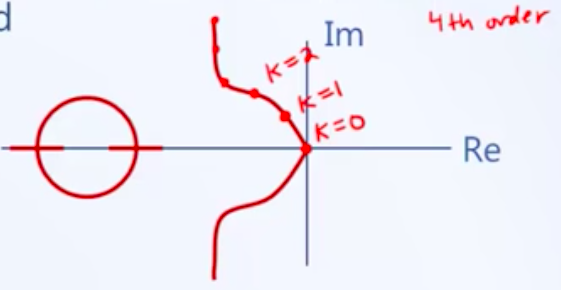
\includegraphics[width=0.6\linewidth]{Bilder/RootLocus_Def}
	\caption{Root locus definition}
	\label{RootLocus_Def}
\end{figure}
The above system is a $4th$ order system with $4$ poles, therefore a complicated higher order system which would be very comple and time consuming with algebriac manipulation using pole placement method. Also with root locus it is possible to find the design control gains very quickly and it provides approximate results quickly (graphically).

\section{Theory on Root Locus}

The theory that describes the origin of root locus that is needed to draw the graphical form of the evolution of system poles with the increasing control gains $K$. This theory in itself is not very important to be known interms of control design perspective, however, the rules that the theory lays down at the end are important to be remenbered. 

The root locus theory states that the evolution of the system poles with respect to control gains can be completely described onlu by using open-loop (OL) system poles and zeros. In order to do so two kinds of constrains are developed by establishing a relationship between the values of $s$ and the control gain $K$. It should also be noted that this theory is nowdays only relavent in order to understant where the root locus of the control system poles originates and would only give a rough approximation in the paper, a better accurate numerial value of root locus can be directly found from Matlab which uses another way to find root locus numeriaclly as described in a later section \ref{Sec_RootLocus_Matlab}. Before develving in the theroy it is important to define open-loop (OL), foward and close-loop (CL) transfer function of a system.

\subsection{OL, forward and CL TF}

Consider a system shown in figure \ref{Fig_OL_forward_CL_TF}, for which OL, forward and CL TF's of the system can be defined as follows:
\begin{figure}[h!]
	\centering
	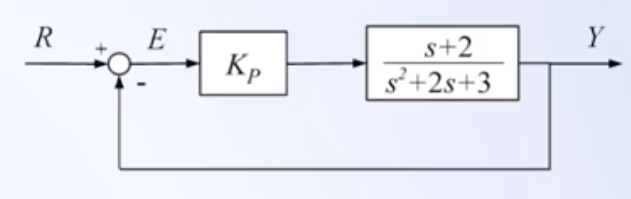
\includegraphics[width=0.6\linewidth]{Bilder/OL_Forward_CL_TF}
	\caption{Root locus definition}
	\label{Fig_OL_forward_CL_TF}
\end{figure}
\textbf{Open-Loop TF}: The OL TF is the TF taken when the summation point is broken off and taking the TF by multiplying all the blocks in the loop just the way thinking that the summation point of the loop is like an output as shown below:
 \begin{equation}
	TF_{OL} = \frac{K_P (s+2)}{s^2 + 2s + 3}
\end{equation}
\textbf{Forward TF}: The forward TF is taken considering only the forward path of the system, therefore, if the system contains sensors in the feedback loop they would be ignored as shwon below (in this example there is no feedback sensor):
\begin{equation}
	Forward_{TF} = \frac{K_P (s+2)}{s^2 + 2s + 3}
\end{equation}
\textbf{Closed-Loop TF}: CL TF is defined using block reduction techniques that are used to calculate the TF of the entire system and the follwoing formula is obtained for a negative CL system:
\begin{equation}
	CL_{TF} = \frac{Forward_{TF}}{1 + TF_{OL}}
\end{equation}

\subsection{Defining the constraint equation for the root locus}

Consider the CL TF for the system shown in figure \ref{Fig_OL_forward_CL_TF}:
\begin{equation}\label{Eq_RootLocus_CL_TF}
	G(s) = \frac{P(s)H(s)}{1 + P(s)H(s)}
\end{equation}
where,
\begin{equation}
	P(s)H(s) = \frac{K_P (s+2)}{s^2 + 2s + 3}
\end{equation}
therefore, the denominator term of equation \ref{Eq_RootLocus_CL_TF} from which the poles of the system can be determined can be written as:
\begin{equation}
	1 + P(s)H(s) = 1 +  K \frac{N(s)}{D(s)}
\end{equation}
where $K$ is taken as the genral control gain of the system. Further using the abouve eqaution a relationship can be established as:
\begin{equation} \label{Eq_RootLocus_Constraint}
	1 +  K \frac{N(s)}{D(s)} \implies \frac{N(s)}{D(s)} = -\frac{1}{K}
\end{equation}
It showed be remembered that the relationship established using equation \eqref{Eq_RootLocus_Constraint} was derived completly using the denominator of equation \eqref{Eq_RootLocus_CL_TF} so that only the description of the poles is obtained w.r.t to the control gain $K$. Equation \eqref{Eq_RootLocus_Constraint} form the constraint eqaution that was previosuly described in the introduction.

The common gain of the system can be also be determined using the following way. Suppose a PID controller is used in series with a plant PT-1:
\begin{align*}
	G(s) = C(s)P(s) &= K_P + \frac{K_I}{s} + K_D s \left( \frac{1}{\tau s + 1} \right) \\
	G(s) &= \frac{K_P s + K_I + K_D s^2}{s} \left( \frac{1}{\tau s + 1} \right) \\
	G(s) &= K \frac{s + K_I^{*} + K_D^{*} s^2}{s(\tau s + 1)} = K \frac{N(s)}{D(s)}
\end{align*}
where, $K_I^{*} = K_I / K_P$ and $K_D^{*} = K_D / K_P$. This is just for an example ,the factor $K$ could also have been chosen for $K_D$.

\subsubsection{Constraint 1}

From equation \eqref{Eq_RootLocus_Constraint}, it should be seen that for the ration on the $RHS - 1 / K$ is satisfied iff the vale of $s$ satisfies the ratio on the $LHS = N(s)/D(s)$. In other words, there are only a certain definite values of $s$ for which the ratio $-1 / K$ is satisfied and also the vice-versa that the control gain $K$ only satifies the root locus for a certaint values of $s$.

\subsubsection{Constraint 2}

If the constraint equation \eqref{Eq_RootLocus_Constraint} is used to plot on the complex plane, the constraint ratio $-1/K$ can be plotted as shown in figure \ref{Fig_RootLocus_ConstPlot}.
\begin{figure}[h!]
	\centering
	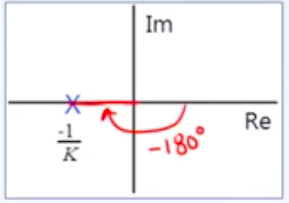
\includegraphics[width=0.6\linewidth]{Bilder/RootLocus_ConstraintPlot}
	\caption{Root locus constraint ratio plot on the complex plane}
	\label{Fig_RootLocus_ConstPlot}
\end{figure}
As the ratio is negative and lies on the real axis the position is plotted as shown at $-1 / K$ in figure \ref{Fig_RootLocus_ConstPlot}. The position $-1 / K$ should have some magnitude and direction if it can be seen through polar corrdinates just like the poles that have magnitude $\omega_{n}$ and direction $\cos{\beta}$ w.r.t negative real axis. Therefore, a new constraint relationship can be extablished now using such magnitude and angle constraints. In polar coordinates the angle is measured w.r.t the positive real axis as shwon in figure \ref{Fig_RootLocus_ConstPlot}, also it can be seem that these angles are repeating for every $180^{\circ}$ weather it is approached from as $+ \theta$ or $- \theta$ from the positive real axis. Therefore, a new constraint can be formed using angle constraint on the ratio $-1 / K$ as given below:
\begin{equation}
	\angle \frac{N(s)}{D(s)} = 180^{\circ} \pm 360^{\circ} n
\end{equation}
where $n = 0,1,2,3...$. Further, the magnitude is quite straight-forward and it shpuld be expressed as:
\begin{equation}\label{Eq_RootLocus_MagConst}
	\left|\frac{N(s)}{D(s)} \right| = \frac{1}{K}
\end{equation}
Further, using the magnitude constraints, the following conclusions can be drwan and the first of the few rules of root locus can be laid down. Generally, in a TF of the form $\frac{N(s)}{D(s)}$, the values of $s$ for which the denominator goes to zero are called poles and similarly the values of $s$ for numerator can be defined as zeros. Now we have a relationship of $\frac{N(s)}{D(s)}$ which was originally taken from the denominator of equation \ref{Eq_RootLocus_CL_TF} such that the poles from manipulated equation $\frac{N(s)}{D(s)}$ alternate themselves between further values of poles and zeros as explained further.

In case $K = 0$ in eqaution \eqref{Eq_RootLocus_MagConst}, the ration $\rightarrow \infty$, therefore, $\frac{N(s)}{D(s)} \rightarrow \infty$. For this to be true $D(s) \rightarrow 0$. The values of $s$ for whih the denominator $D(s) \rightarrow 0$ are called poles. If $s$ has the value of poles, then it should have been the value without $K$ into consideration. A pole value without $K$ taken into consideration is alo the OL pole where $K = 0$. Therefore, the root locus approaches the OL poles (see section \ref{Sec_RootLocus_Matlab} how this happens numerically). Similarly, for the condition that $K \rightarrow \infty$, the ratio $\frac{N(s)}{D(s)} \rightarrow 0$, for this condition $N(s) \rightarrow 0$. For this condition then the root locus approaches the OL zeros. So it can be seen that the root locus starts from OL poles and terminates ar OL zeros (first rule of root locus). This also proves the facts that the root locus can be drawn using only the OL TF of the system, as was this mathematical (strangely wierd) derivation of root locus began with. 

Lastly, it should also be noted that when there are more ploes than zeros, then this includes zeros (where $zeros = \# poles - \# zeros$) that approach infinity (aslo called asymptotes).

\subsection{Rules for drawing rot locus}

The following rules are genrerally requried to draw a root locus:
\begin{enumerate}
	\item Locate the OL poles and zeros in the s-plane
	\item Determine root locus on the real axis
	\item Approximate the asymptotes of the root locus
	\item Approximate the break-away and break-in points
	\item Determine angles of departure and arrival
	\item Find imaginary angle crossings
\end{enumerate}
On pen and paper, it is only possible to draw a rough scketch of the root locus, it is a better practice to use Matlab for all kinds of root locus calculations as this mehtod is more suited numerially but analytically. A rought idea of how the root locus looks like can be drwan on the paper just to get an idea but the precise root locus with all its properties is only possible using Matlab.

\subsection{Root locus using Maltab} \label{Sec_RootLocus_Matlab}

Matlab uses a brute force calculation of root locus determination using numerical calculations rather using the analytical approach as described in the previous section. A numerical approach for calculating is better suited approach as it is only possible numerically to obtain a better precision than analytially drwaing on tools such as graphs. Consdier the system shown in figure \ref{Fig_OL_forward_CL_TF} again, the OL and CL TF can be expressed as:
\begin{align}
	G_{OL} &= \frac{K_P}{s^2 + 2s + 3} \\
	G_{CL} &= \frac{K_P(s + 2)}{s^2 + (2 + K_P)s + (3 + 2K_P)}
\end{align}
In Matlab the response of the poles is calculated starting form $K = 0$ to $K \rightarrow \infty$ numerically such as when $K = 0$, the CL denominator becomes:
\begin{equation}
	D(s)_{CL} = s^2 + 2s + 3
\end{equation}
which is equal to the OL denominator, further, with $K = 1$ and $K = 2$, the CL denominator can be expressed as $s^2 + 3s + 5$ and $s^2 + 4s + 7$ respectively. At $K = \infty$, $D(s) = K_Ps + 2 K_P = K_P(s + 2)$ which is equal to the OL zeros. Therefore, it can also be proved numerially that the root locus of a control system starts with OL poles and ends at OL zeros.

\section{Examples of control design with Root Locus}

Steps in control design using Root Locus:
\begin{itemize}
	\item The first thing in the control design is to translate the performace specifications into closed loop pole locations
	\item Draw Root Locus of the system using a simple gain $K$
	\item See if gain change can meet the requirements
	\item If not, then add poles and / or zeros via a controller to reshape the root locus to pass through the desired closed-loop pole locations
\end{itemize}

\subsection{Example: Using a simple P control}

Conider the system as shwon in figure \ref{Fig_RootLocus_Ex_1}. The system has a zero to it, this system however can be approximated to the properties of a PT-2 canonical system. The object is to find the control gain $K$ such that settling time for the system is less than $4/3$$s$.
\begin{figure}[h!]
	\centering
	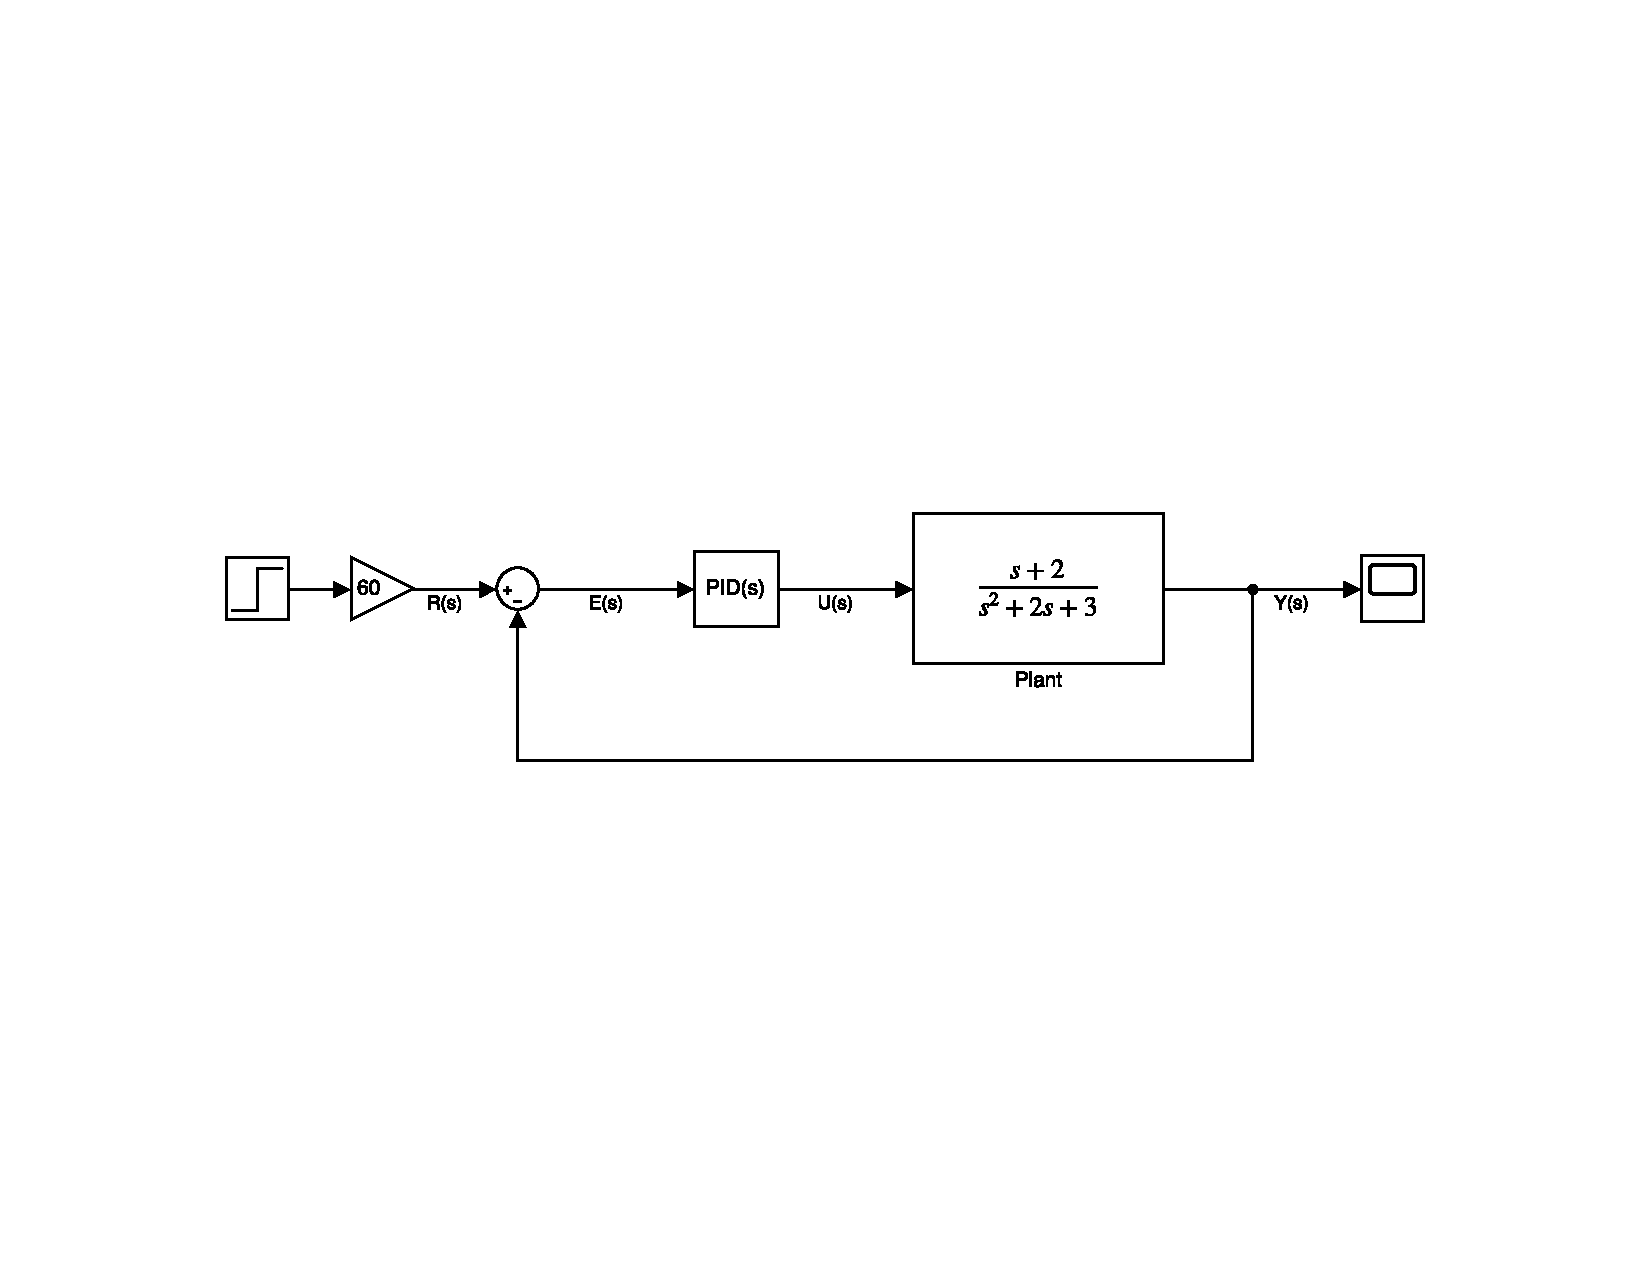
\includegraphics[width=\linewidth]{Bilder/RootLocus_Ex_1.pdf}
	\caption{Control design using root locus (non-canonical systems)}
	\label{Fig_RootLocus_Ex_1}
\end{figure}
Even though the system is not canonical, the control properties can be approximated using the properties from PT-2 system and the control gains found can serve as a starting point in achieving the required control from the given non-canonical system. The setlling time for a PT-2 system is given by:
\begin{equation} \label{Eq_RootLocus_Ex_1_ts}
	t_s \approx = \frac{4}{\sigma} = \frac{4}{3} \implies \sigma = 3
\end{equation}
The root locus of the system is generated using Matlab as shwon in figure \ref{Fig_RootLocus_Ex_1_rLocus}.
\begin{figure}[h!]
	\centering
	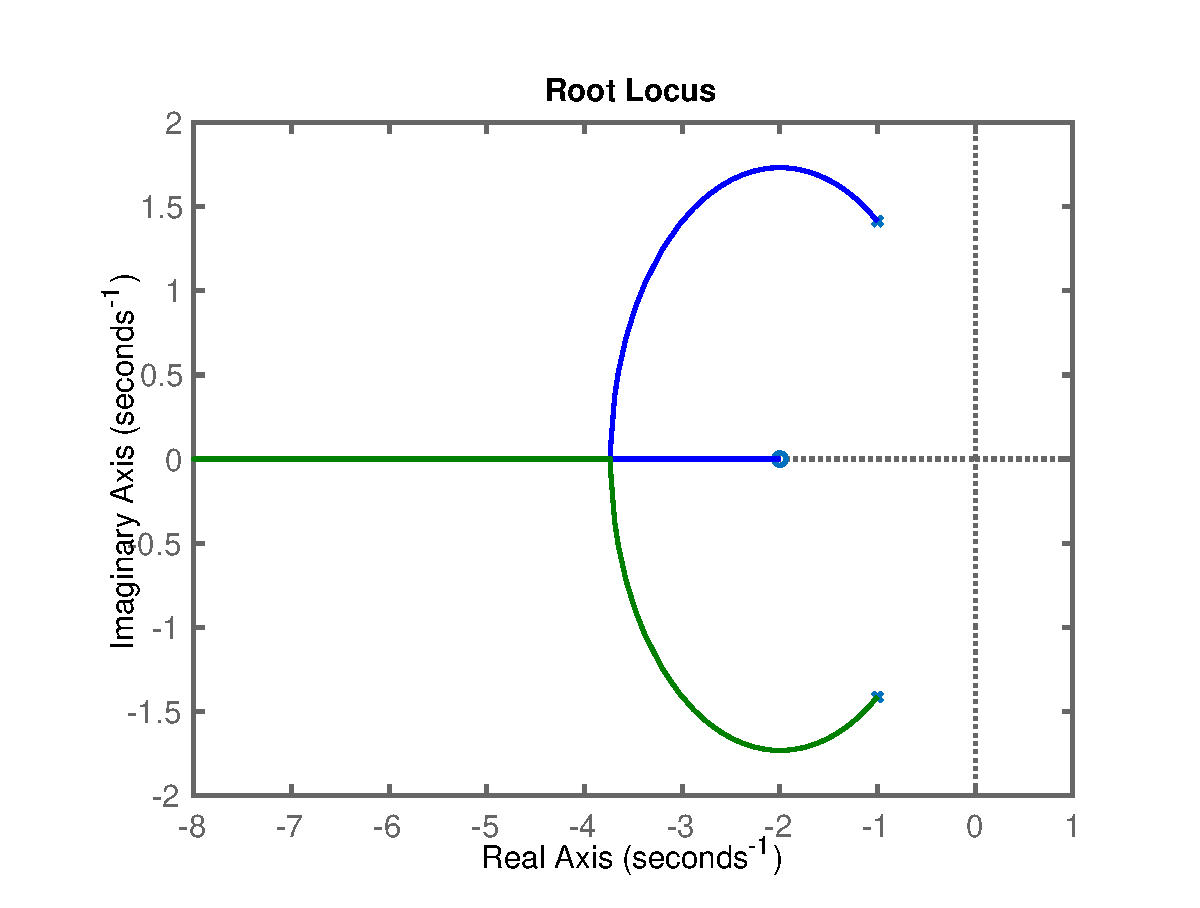
\includegraphics[width=0.7\linewidth]{Bilder/RootLocus_Ex_1_rLocus.eps}
	\caption{Control design using root locus (non-canonical systems)}
	\label{Fig_RootLocus_Ex_1_rLocus}
\end{figure}
As can be seen from equation \eqref{Eq_RootLocus_Ex_1_ts} that the real part of the poles should be $3$ for the conidition to be met. Looking at figure \ref{Fig_RootLocus_Ex_1_rLocus}, it can be seen that this condition is possible at two complex pole location (if we imagine a line drawn through $-\sigma = -3$). So the requirement can be met. It can also be noted that as $K$ is increased, the two poles proceed farther towrads left of $\sigma$, therefore, providing a better settling time. Howeevr, it should also be noted that one of the two poles (blue line) after break-in point proceeds in the directon of increasing $\sigma$ for higher $K$. There are two poles in the system, at higher $K$ the pole with blue line wiill be dominant because of its slower settling time.

Because this system is not exactly a canonical system, the settling time of $4/3$ may be achieved based on the root locus that falls under the value of $-\sigma = -3$. Howeevr, it is always not possible with non-canonical systems to achieve these properties accurately mainly because of the lack of insigths that we have compared to the canonical systems. Using Matlab the following system responses can be generated for a unit step function. For $\sigma = 3$, from Matlab it can be found that $K = 4.07$. The system reponse is found using Matlab again as shown in figure \ref{Fig_RootLocus_Ex_1_sysRes_1}.
\begin{figure}[h!]
	\centering
	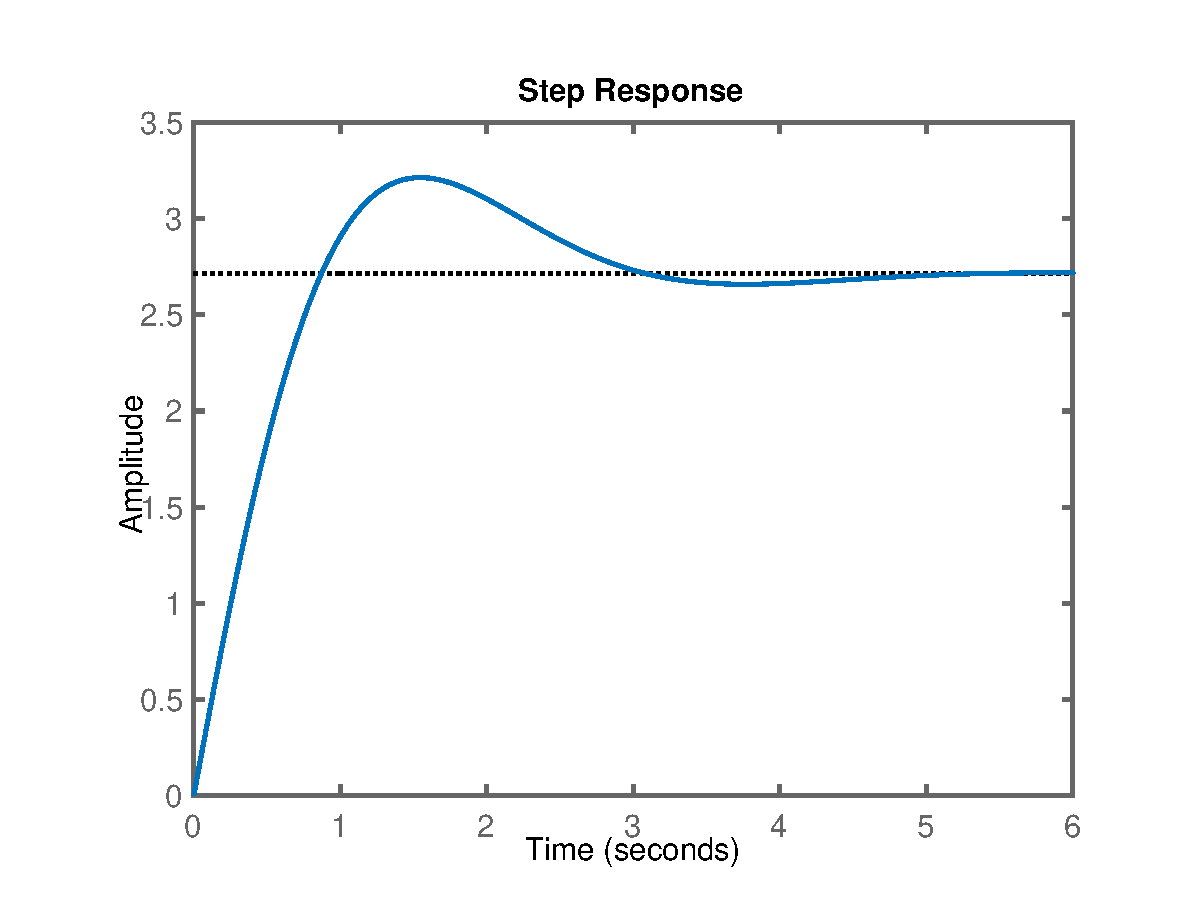
\includegraphics[width=0.7\linewidth]{Bilder/RootLocus_Ex_1_Res_1.eps}
	\caption{System response for $K = 4.07$}
	\label{Fig_RootLocus_Ex_1_sysRes_1}
\end{figure}
\newpage
Further increasing gain $K = 5.46$ such that $-\sigma = -3.73$, the following system response was generated given in figure \ref{Fig_RootLocus_Ex_1_sysRes_2}.
\begin{figure}[h!]
	\centering
	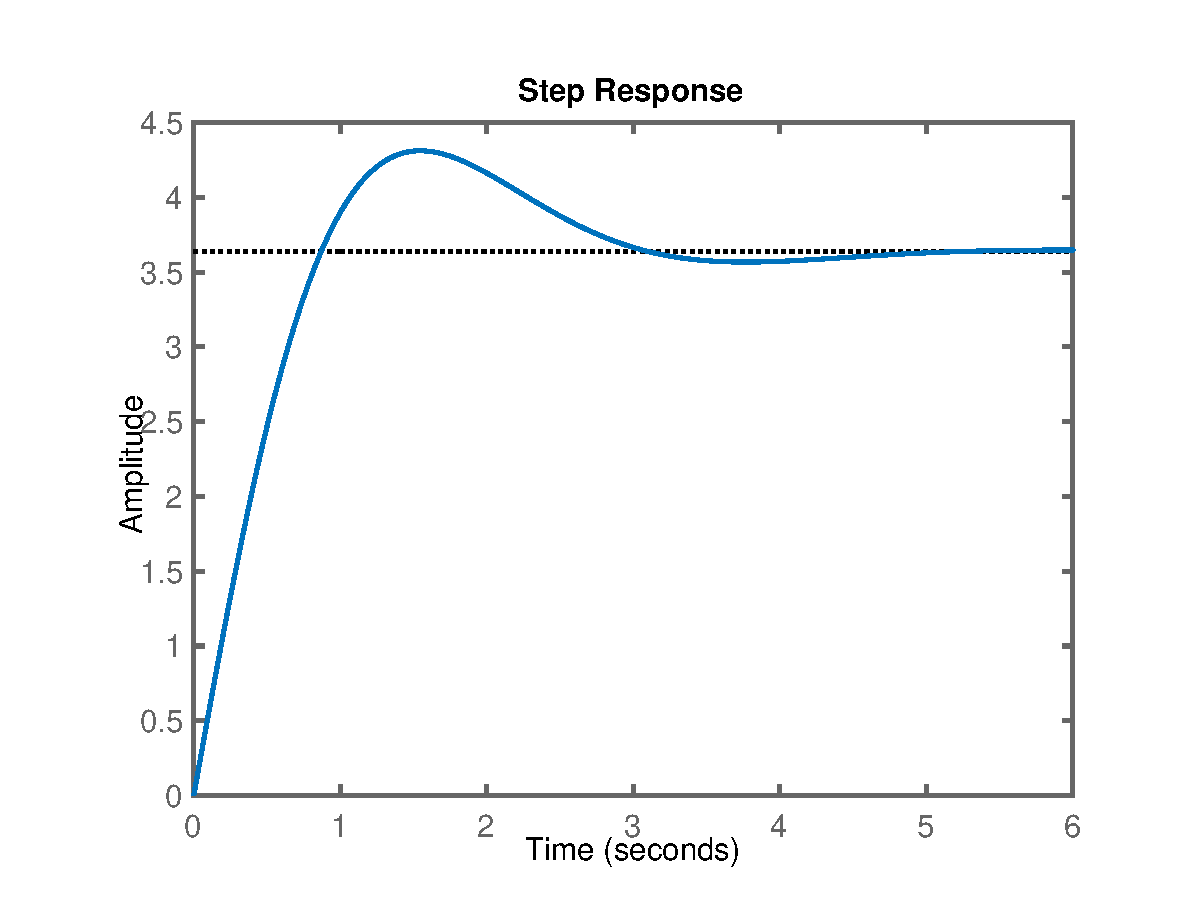
\includegraphics[width=0.7\linewidth]{Bilder/RootLocus_Ex_1_Res_2.eps}
	\caption{System response for $K = 5.46$}
	\label{Fig_RootLocus_Ex_1_sysRes_2}
\end{figure}
\newpage
Clearly, from both the figure (\ref{Fig_RootLocus_Ex_1_sysRes_1} and \ref{Fig_RootLocus_Ex_1_sysRes_2}), it can be seen that the required system response is not achieved, this is all because of a single zero that is present in the system due to which it would be not possible from the $\sigma$ value calculated using \eqref{Eq_RootLocus_Ex_1_ts} which is actually an approximated value for $t_s$ of a PT-2 system.

\subsection{Example: Altering root locus using I or D poles or zeros}

Consider a PT-2 system in series intially with a P control as shown in figure \ref{Fig_RootLocus_Ex_2_sys}. The objet here is to achieve a peak time of less than 1 sec and overshoot less than 4 \%.
\begin{figure}[h!]
	\centering
	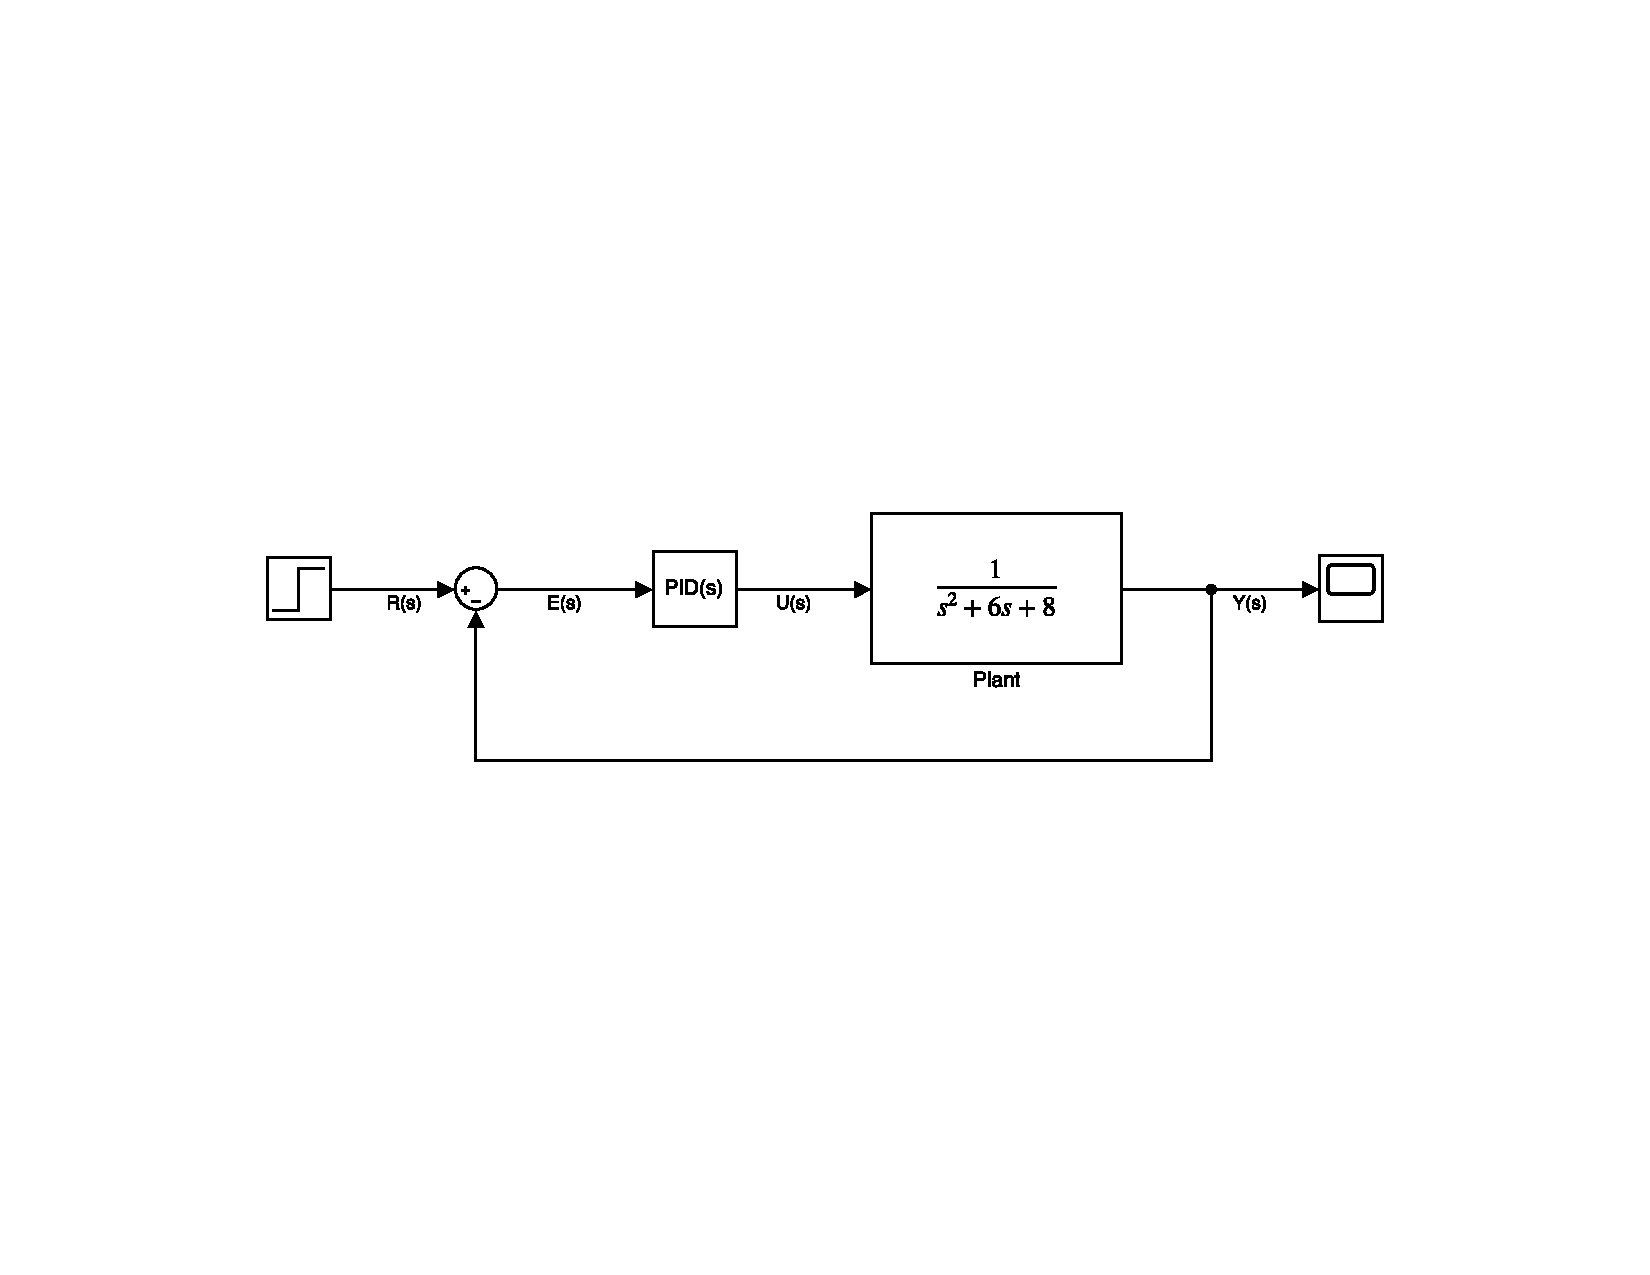
\includegraphics[width=\linewidth]{Bilder/RootLocus_ControlDesign.pdf}
	\caption{Example using root locus altering for this system}
	\label{Fig_RootLocus_Ex_2_sys}
\end{figure}
As this is a PT-2 system, the system properties formalae for the PT-2 system can be used for finding frequency $\omega_{n}$ and damping ratio $\zeta$ (to find the area under root locus which actually produces desired results) :
\begin{equation}
	t_p = \frac{\pi}{\omega_{d}} < 1 \implies \omega_{d} > \pi
\end{equation}
\begin{equation}
	M_p = e^{-\zeta \pi / \sqrt{1 - \zeta^2}} < 0.04 \implies \zeta > \sqrt{\frac{ln(0.04)^2}{\pi^2 + ln(0.04)^2}} \approx 0.707
\end{equation}
also the angle $\beta$ will provide the area under the root locus that of interest in this problem:
\begin{equation}
	\cos{\beta} = \zeta \implies \beta = \cos^{-1}{\zeta} \implies \beta \leq 45^{\circ}
\end{equation}

Plotting this root locus on Malab with the parameters that determine the area under the root locus important $\omega_{n} \quad \zeta \quad \beta$, the root locus is as shown in figure \ref{Fig_RootLocus_Ex_2_rLocus}.
\begin{figure}[h!]
	\centering
	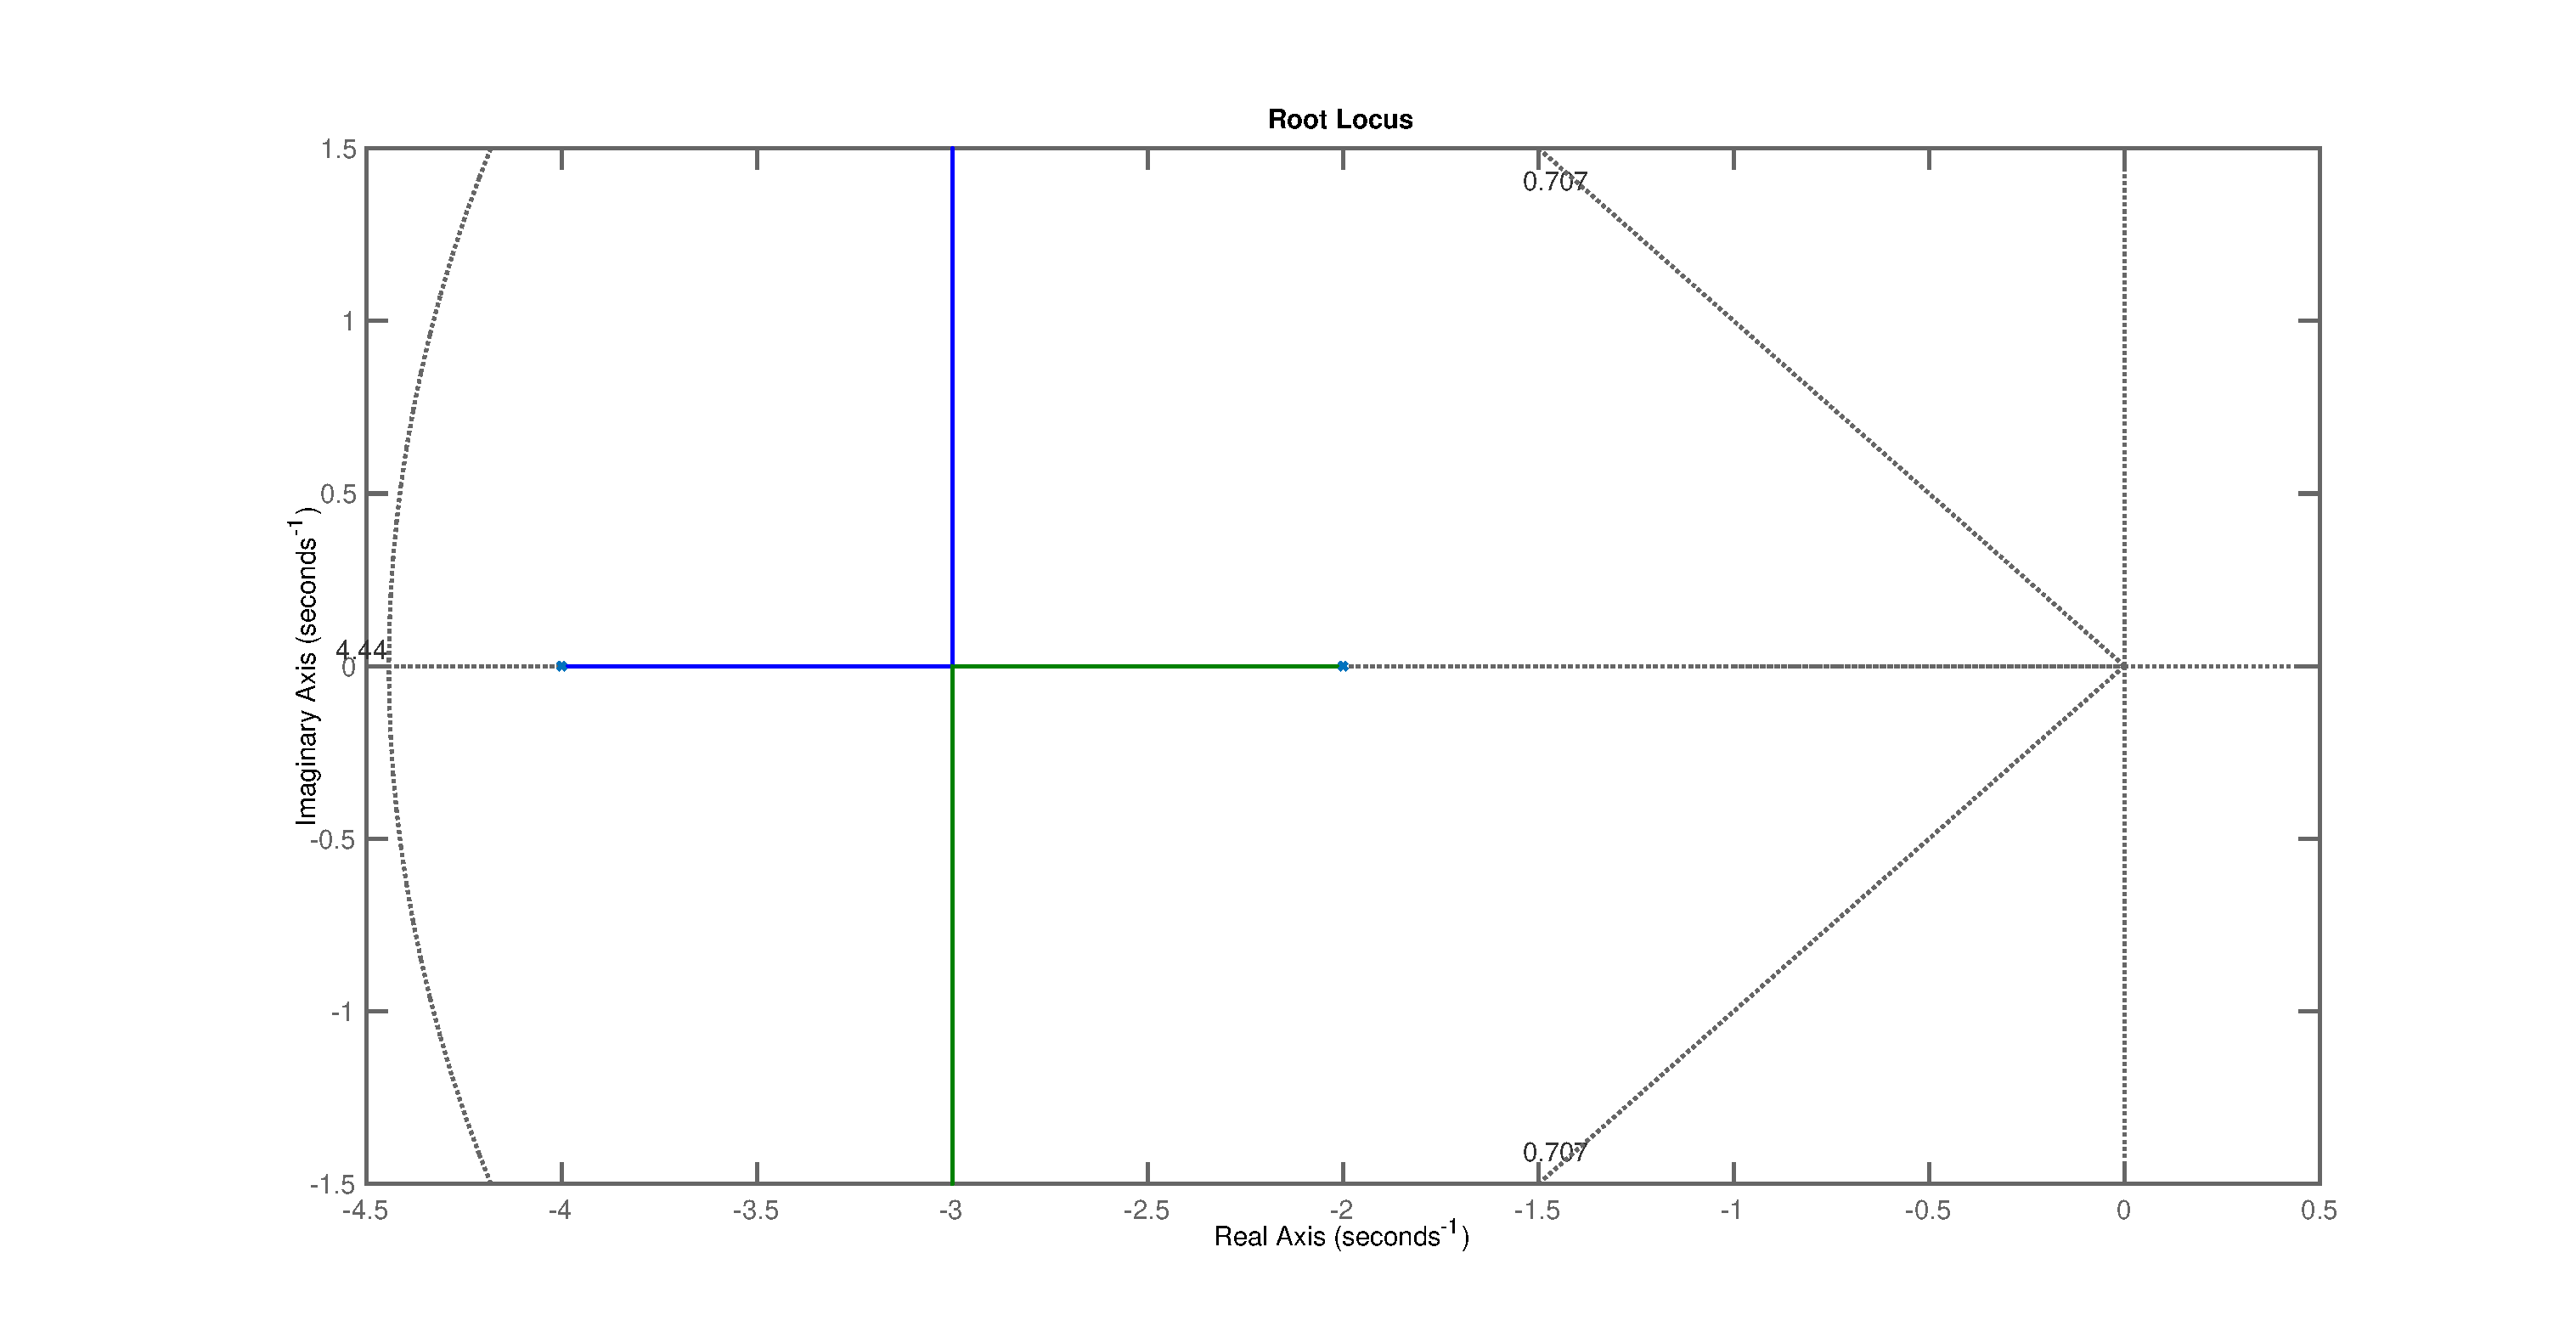
\includegraphics[width=\linewidth]{Bilder/RootLocus_ControlDesign_rLocus.eps}
	\caption{Root locus with area of control interest enveloped between semi-circle and angled lines}
	\label{Fig_RootLocus_Ex_2_rLocus}
\end{figure}
\newpage
As can be seen from figure \ref{Fig_RootLocus_Ex_2_rLocus}, the $45 \%$ angles lines are from the value $\beta$, the area under which $\beta < 45 \%$ (required). The semi-circle denotes the line on which $\omega_{n} = 4.44 rad/s$, the area over this line is when $\omega_{n} > 4.44$ (required). It can be seen that this area does not cover the existant root locus, therefore, there is a need to add either a differential or an integral control either to add poles or zeros. By observing figure \ref{Fig_RootLocus_Ex_2_rLocus}, it can be seen that the poles are proceeding to $\infty$, the required area is to the left of the existing root locus, therefore, a firs attempt would be to try to bend the poles that are pointing to $\infty$ towards the left of the existing root locus. One way to do this is by adding a zero which will bend the poles pointing to $\infty$ towards the left side where it is required. A D control is therefore employed in the first attempt. 

Writing the PD control,
\begin{equation} \label{Eq_RootLocus_AddSimplePole}
	C(s) = K_D s + K_P = K (s + z)
\end{equation}
where, $z = K_P / K_D$. From equation \eqref{Eq_RootLocus_AddSimplePole}, it can be seen that the location of zero is decided by $s = -z$, so through an iterative approach it can be decided how far the zero location can be placed (value of $z$) in order to achieve desired performace. Looking at the root locus \ref{Fig_RootLocus_Ex_2_rLocus}, we have two poles, there are three positions where a simple zero can be placed as shown below.
\subsubsection{Case 1: Zero to the right of two poles}

Suppose the zero is placed to the right of two poles, such that $s = -1$. The new root locus generated with Matlab can be seen from figure \ref{Fig_RootLocus_ControlDesign_PD1}.
\begin{figure}[h!]
	\centering
	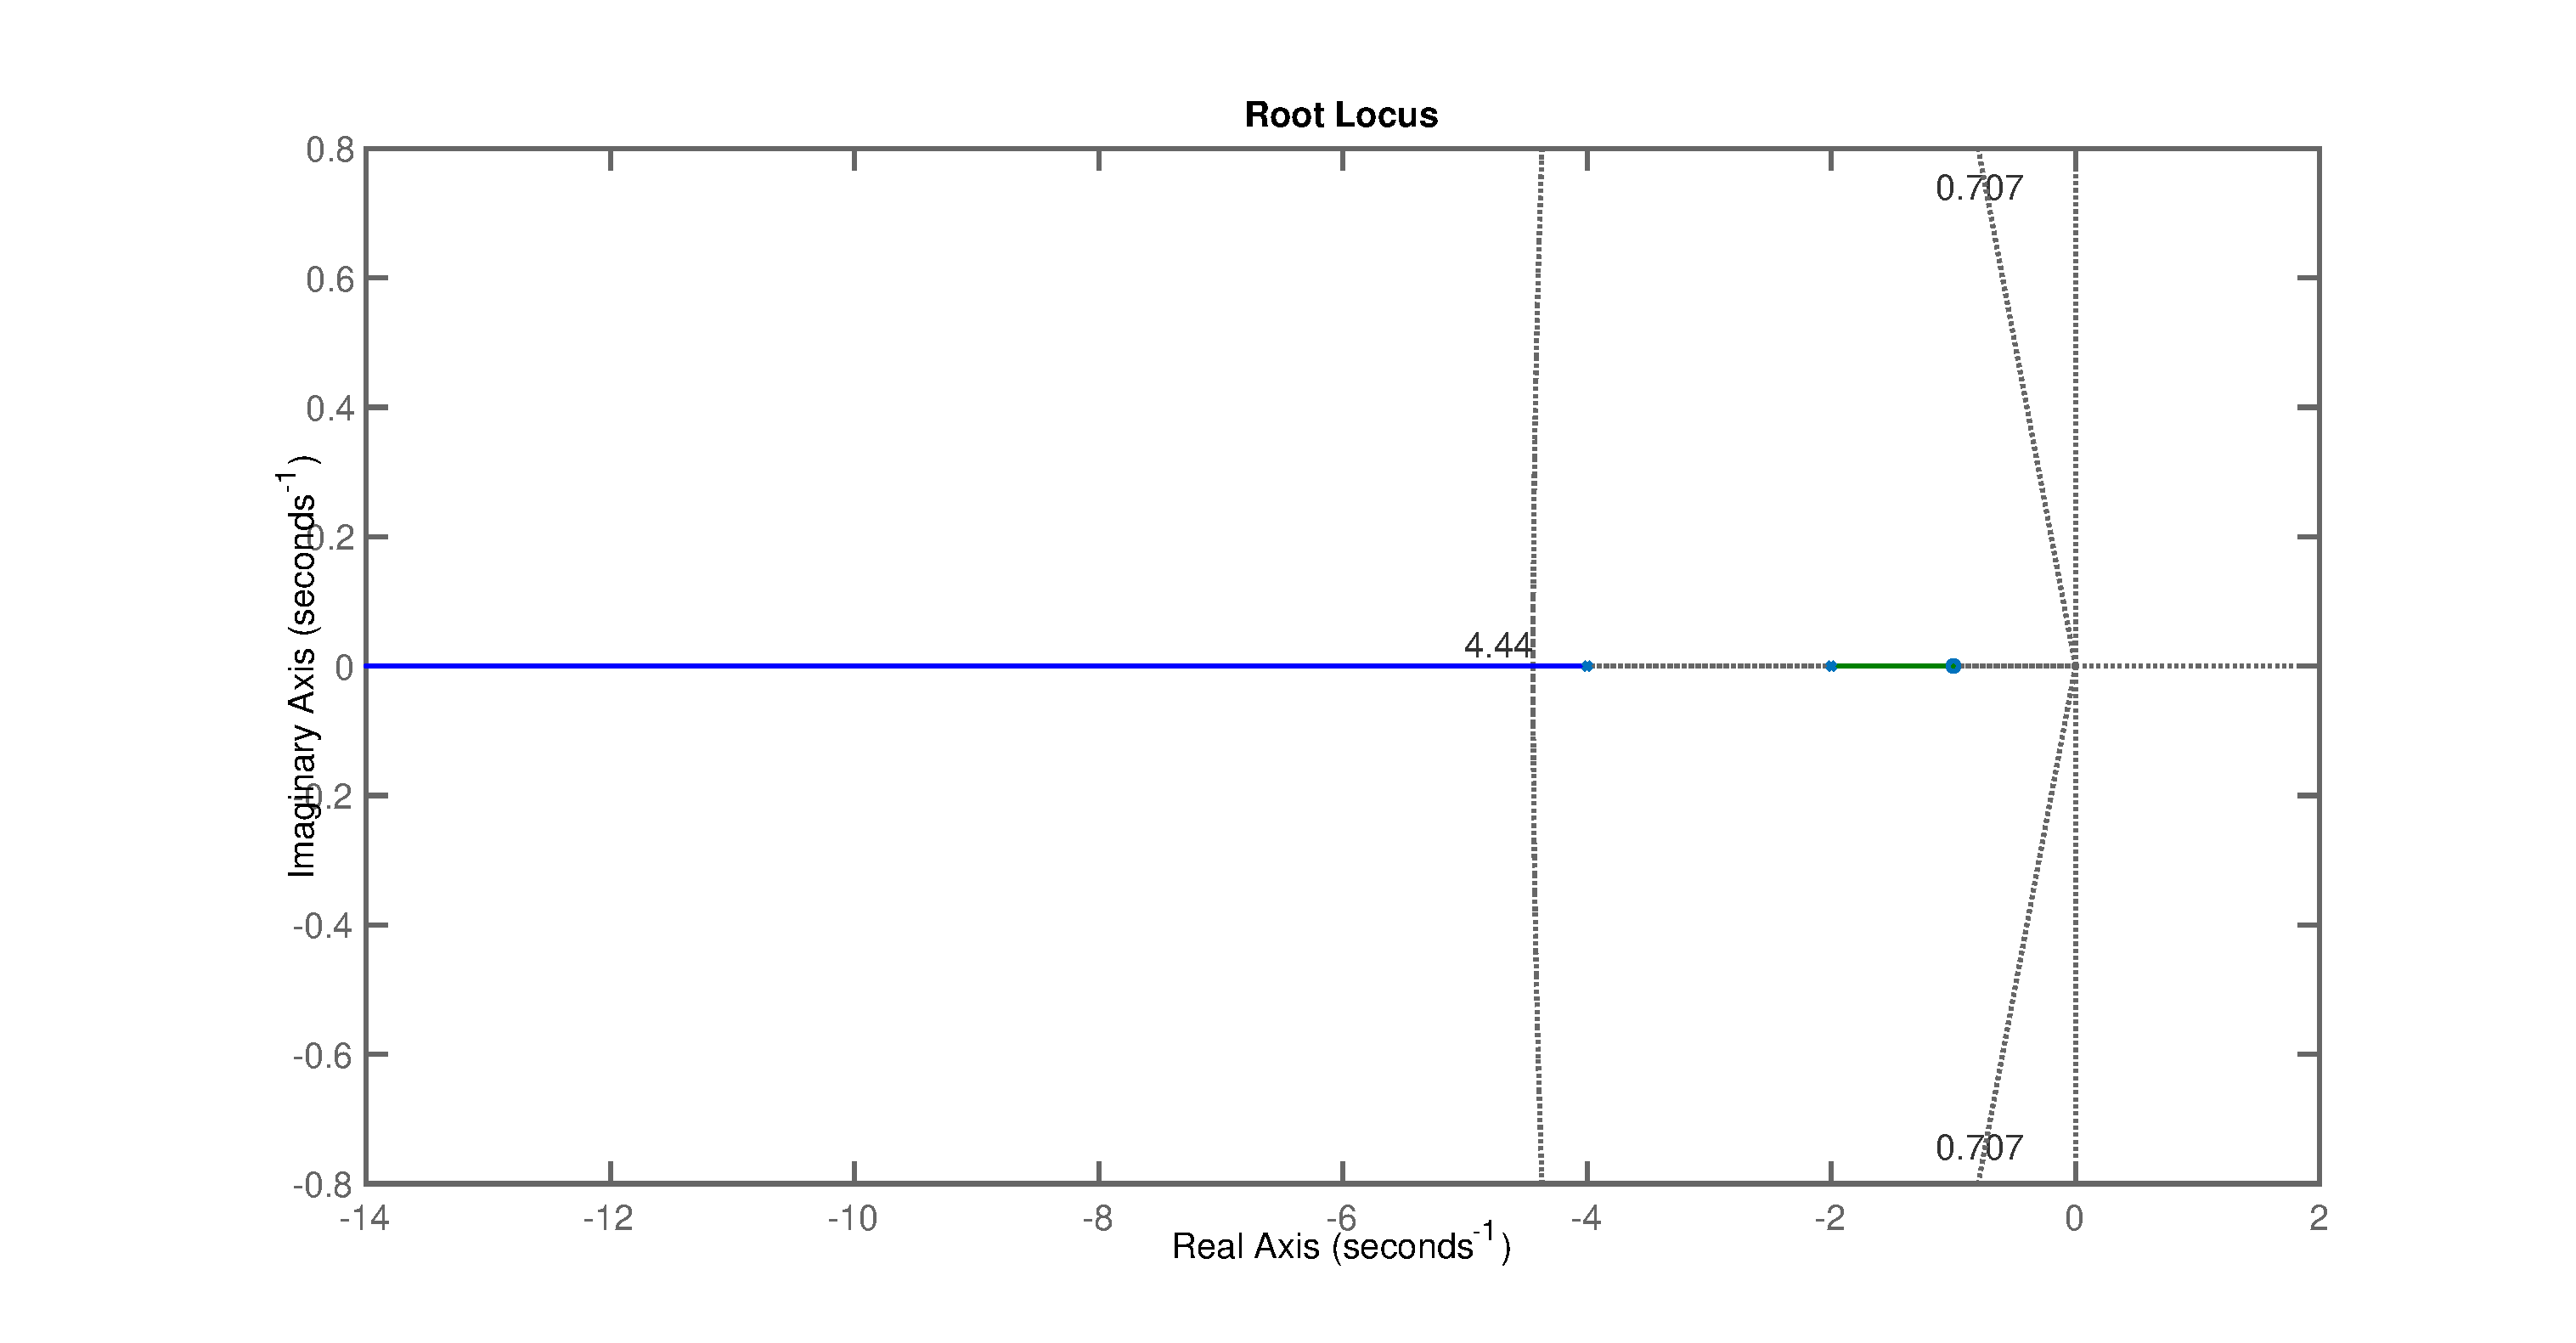
\includegraphics[width=\linewidth]{Bilder/RootLocus_ControlDesign_PD1.eps}
	\caption{Altering root locus by placing a zero to the left of two poles}
	\label{Fig_RootLocus_ControlDesign_PD1}
\end{figure}
\newpage
It can be seen from figure \ref{Fig_RootLocus_ControlDesign_PD1}, it can be seen in this case that even though the root locus lies in the desrired are (blue line), the dominant pole (green line) does not lie in the deisred region. The dominant pole will dominate the response of the system and its root locus does not lie in the requried area for the desired control. Therefore, this case will be rejected.

\subsubsection{Case 2: Zero in between two poles}
For a zero to be inbetween two poles, suppose that $s = -3$, from Matlab the following root locus with the desrired area can be generated as shwon in figure \ref{Fig_RootLocus_ControlDesign_PD2}.
\begin{figure}[h!]
	\centering
	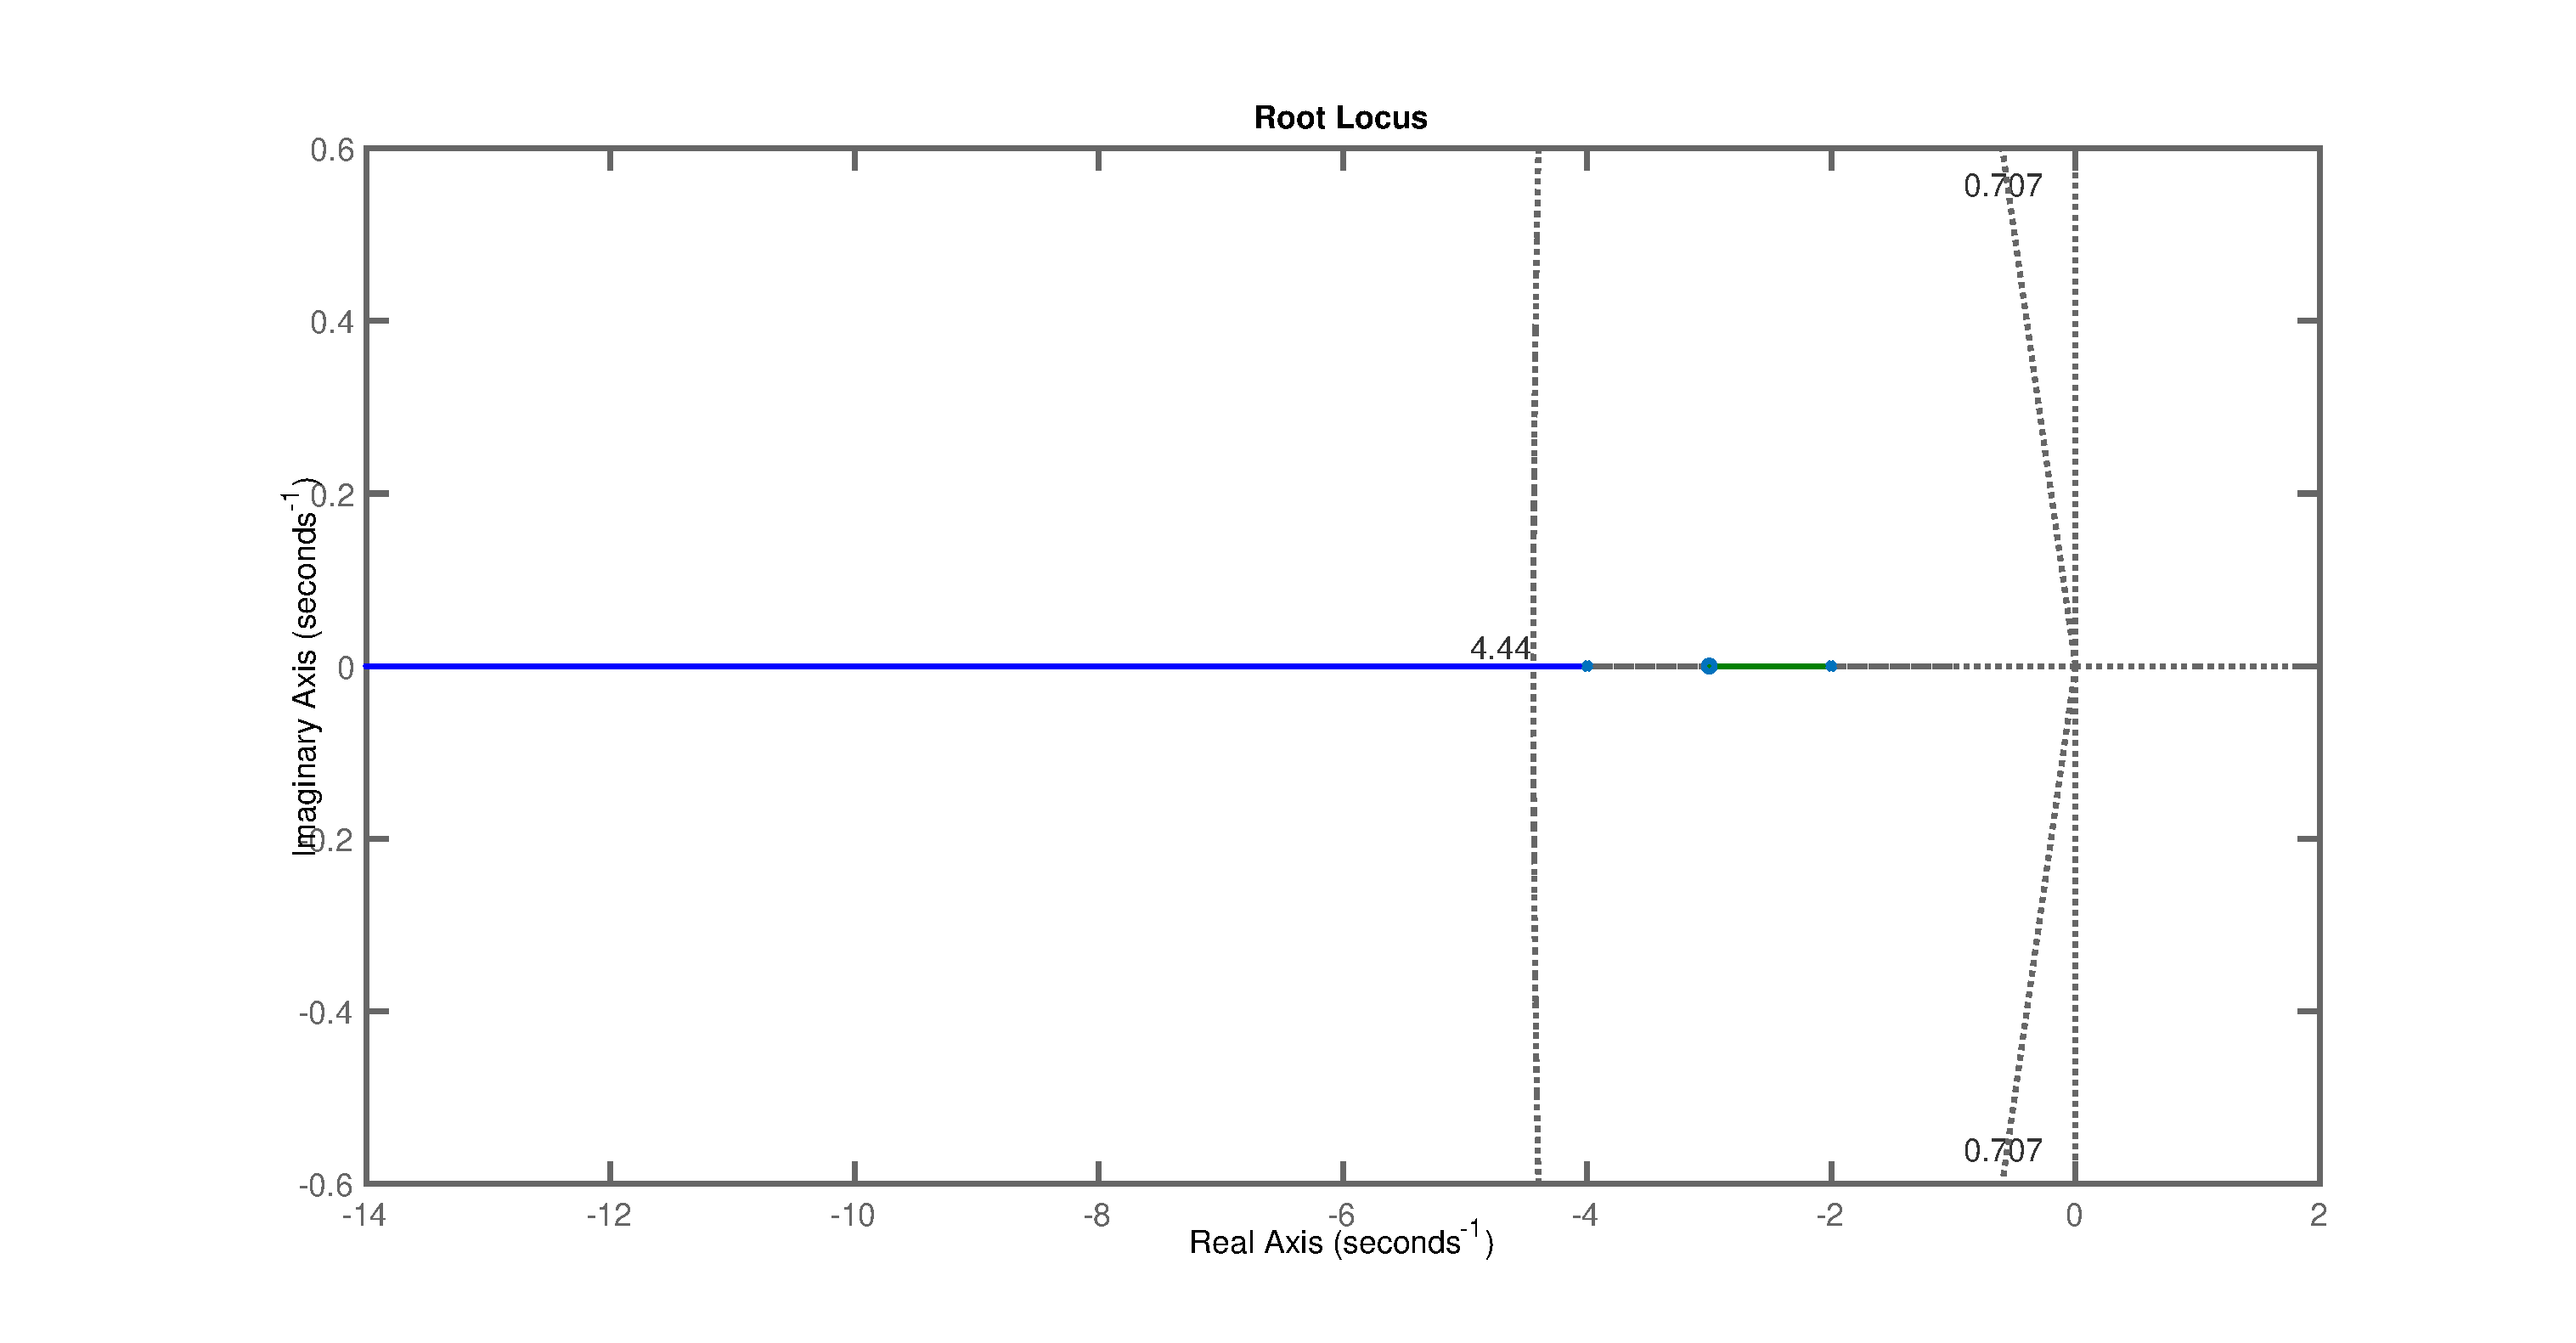
\includegraphics[width=\linewidth]{Bilder/RootLocus_ControlDesign_PD2.eps}
	\caption{Altering root locus by placing a zero in-between two poles}
	\label{Fig_RootLocus_ControlDesign_PD2}
\end{figure}
\newpage
Again in this case the result in same as the result of case 1;

\subsubsection{Case 3: Zero to the left of two poles}
For a zero to the left of two poles, suppose that $s = -5$, from Matlab the following root locus with the desrired area can be generated as shwon in figure \ref{Fig_RootLocus_ControlDesign_PD3}.
\begin{figure}[h!]
	\centering
	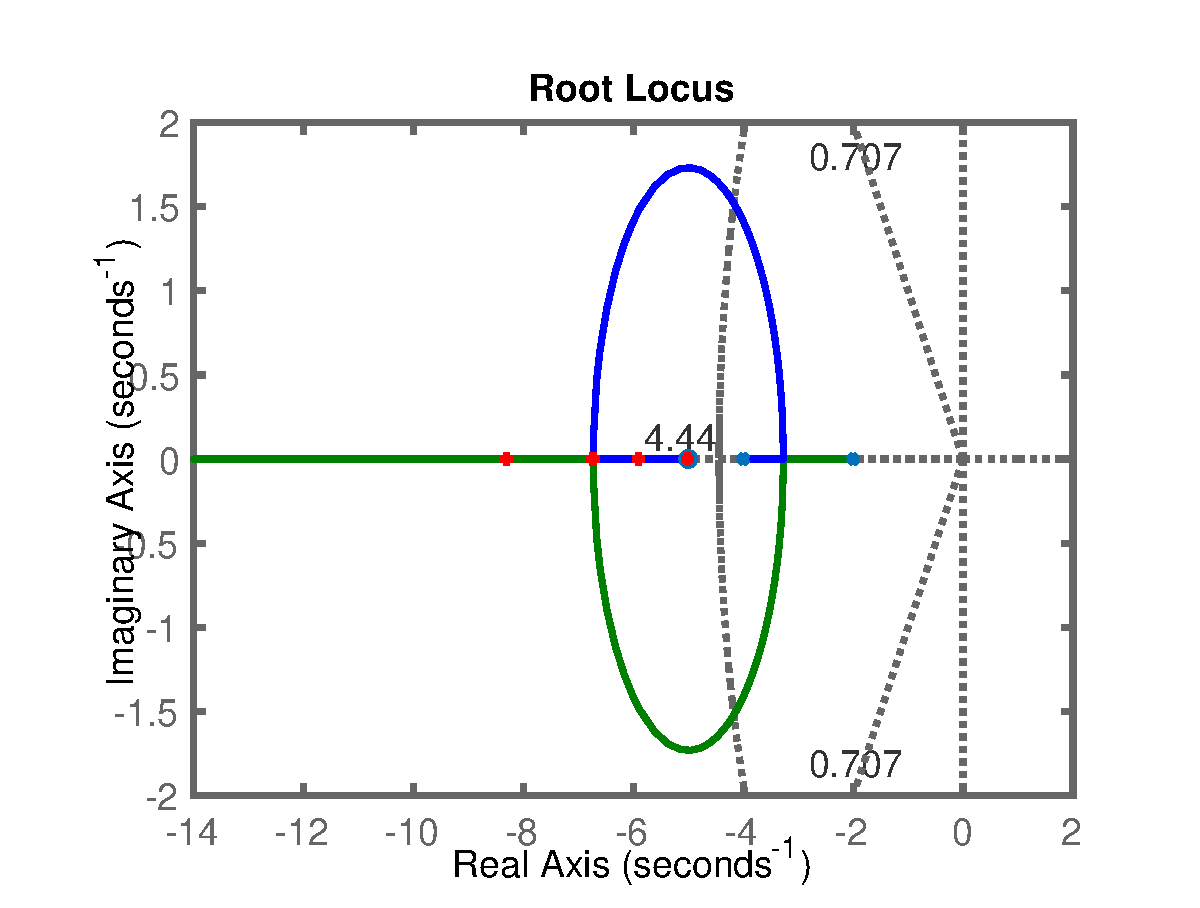
\includegraphics[width=\linewidth]{Bilder/RootLocus_ControlDesign_PD3.eps}
	\caption{Altering root locus by placing a zero in-between two poles}
	\label{Fig_RootLocus_ControlDesign_PD3}
\end{figure}
\newpage
Finally, with this case, the dominant pole lies inside the design area for control (shown by red dots on the blue line). Therefore, the control equation \eqref{Eq_RootLocus_AddSimplePole} can be set to:
\begin{equation}
	C(s) = K(s + 5)
\end{equation}
Using Matlab function [k,poles] = rlocfind(sys), the system gain $K$ for which all the control properties that match the desired requirements can be found, which is found to be at maximum gain $K = 224.84$ therefore, the new poles will now be at $\{s_1,s_2\} = \{225.84, 5.01\}$ for the chosen gain $K$. The step resposne of the system without any control is as shown in figure \ref{Fig_RootLocus_ControlDesign_SysResp}.
\begin{figure}[h!]
	\centering
	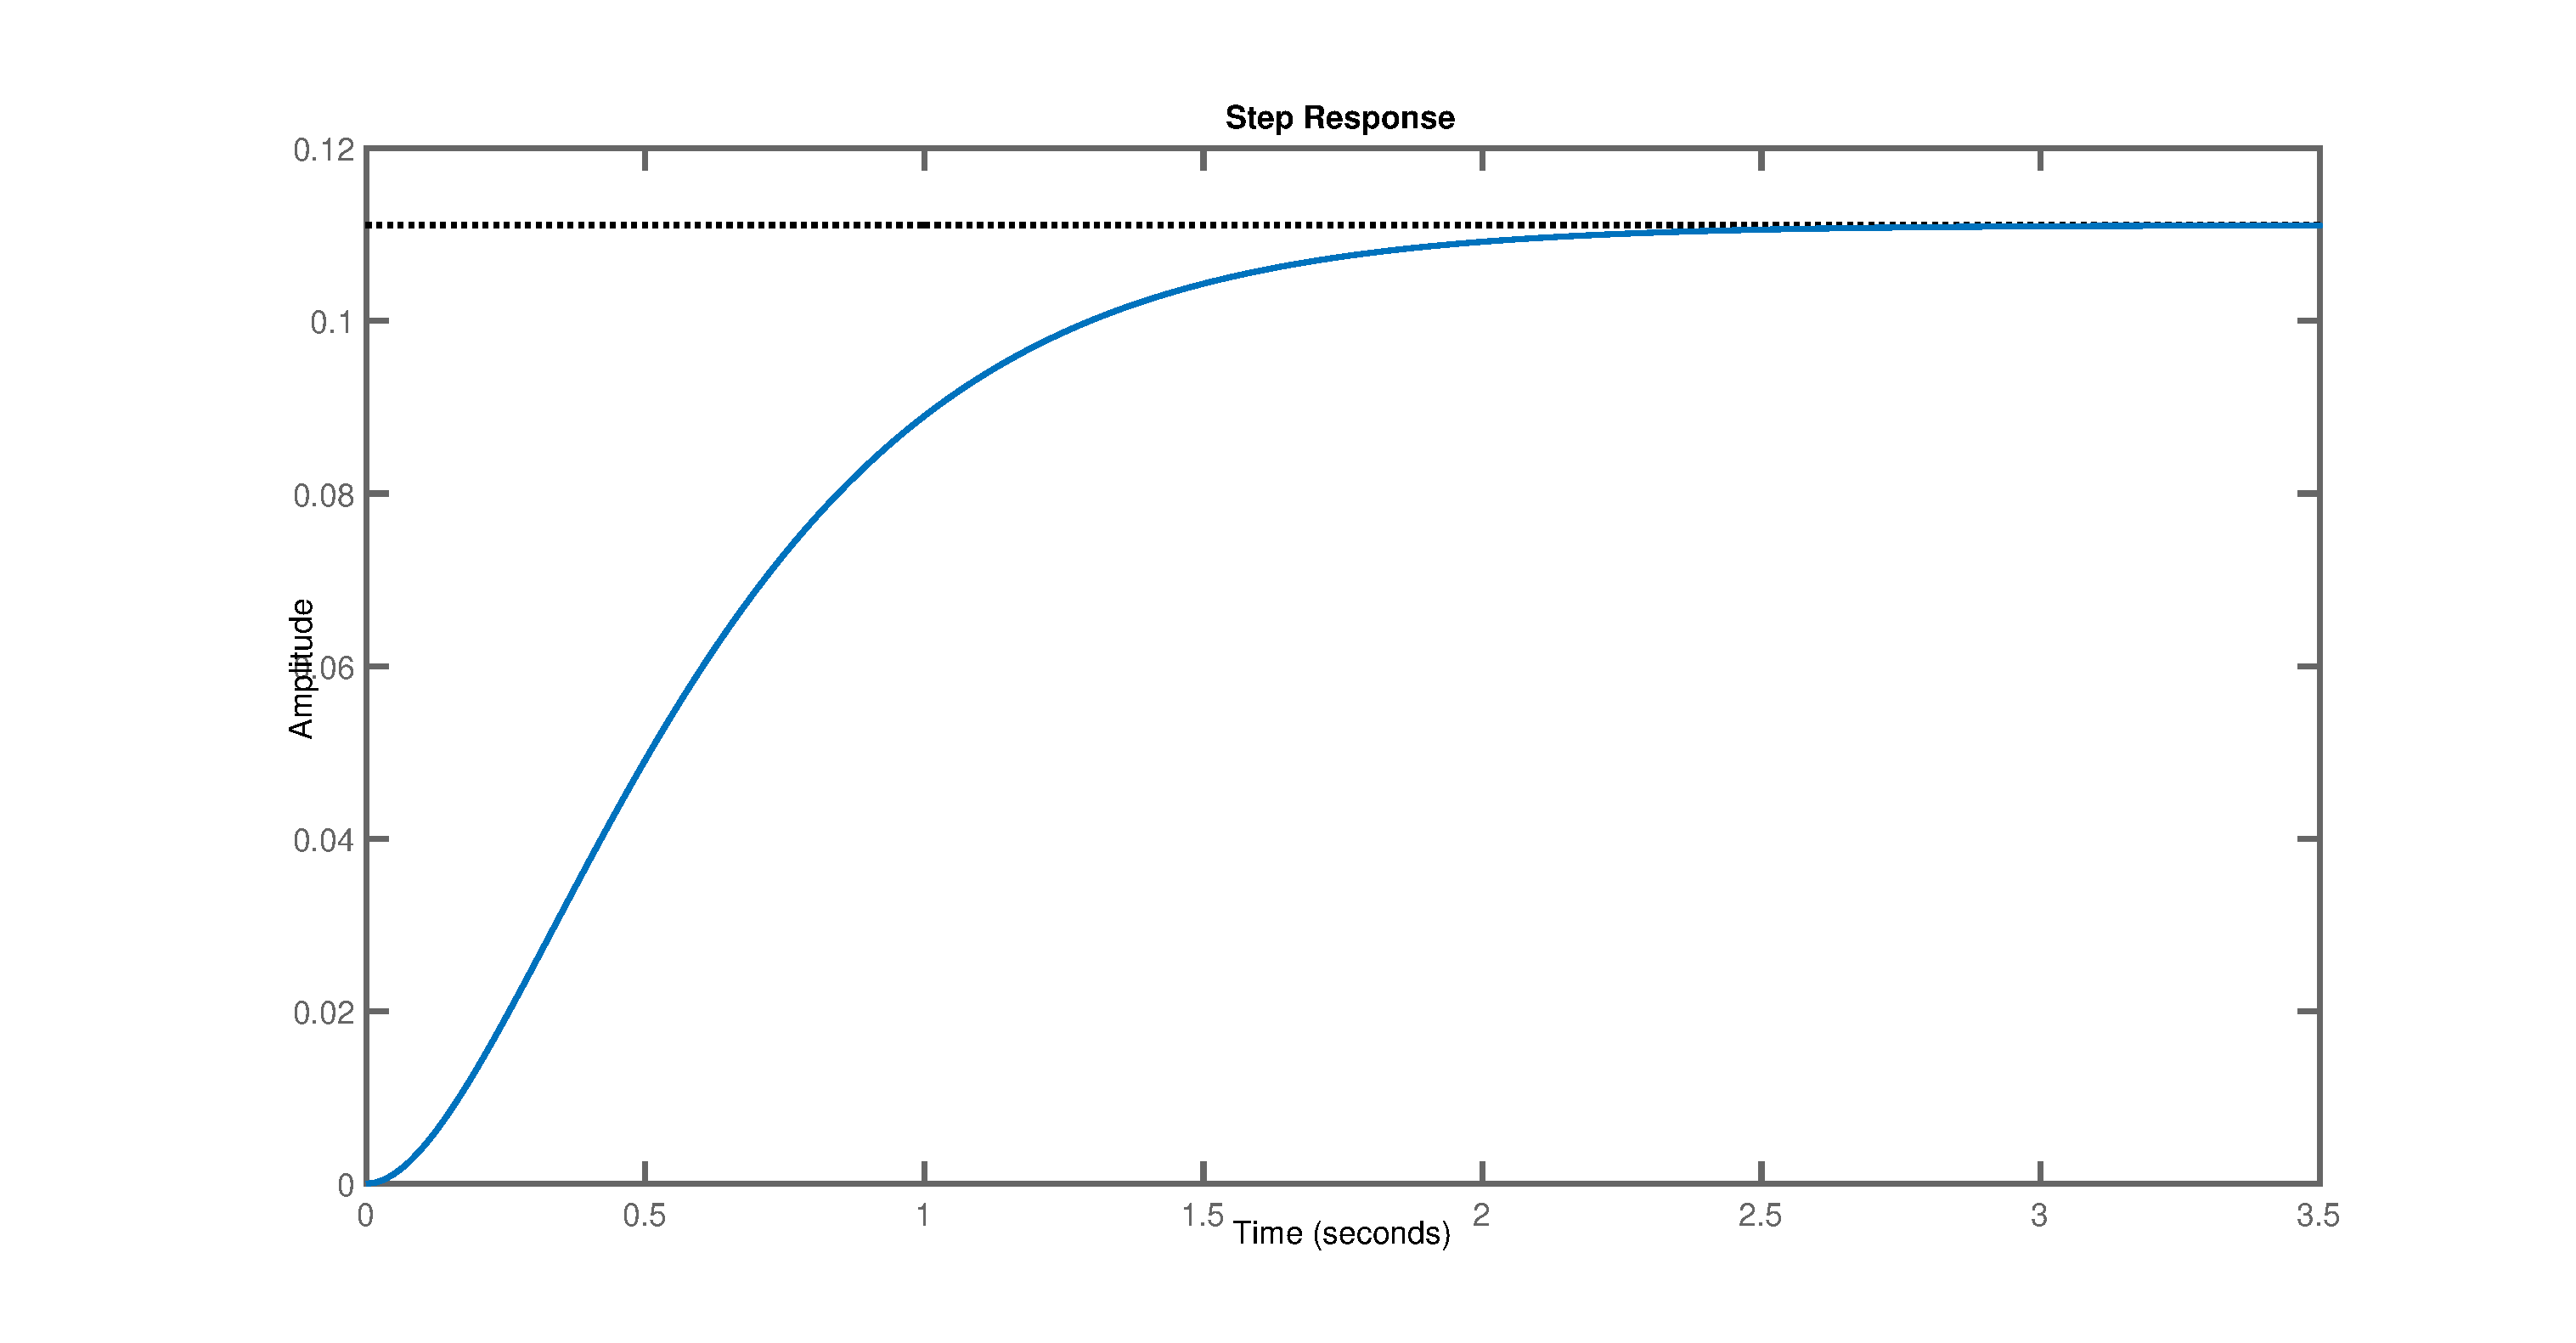
\includegraphics[width=\linewidth]{Bilder/RootLocus_ControlDesign_SysResp.eps}
	\caption{Altering root locus by placing a zero in-between two poles}
	\label{Fig_RootLocus_ControlDesign_SysResp}
\end{figure}
\newpage
It can be seen from figure \ref{Fig_RootLocus_ControlDesign_SysResp}, that the closed loop step response of $G$ has a rise time greater than $1$, which needs to be controlled. Therefore, now with the control design by placing a zero into the system as shown in the above description, a new step response can be plotted using Matlab as shwon in figure \ref{Fig_RootLocus_ControlDesign_SysResp_C}.
\begin{figure}[h!]
	\centering
	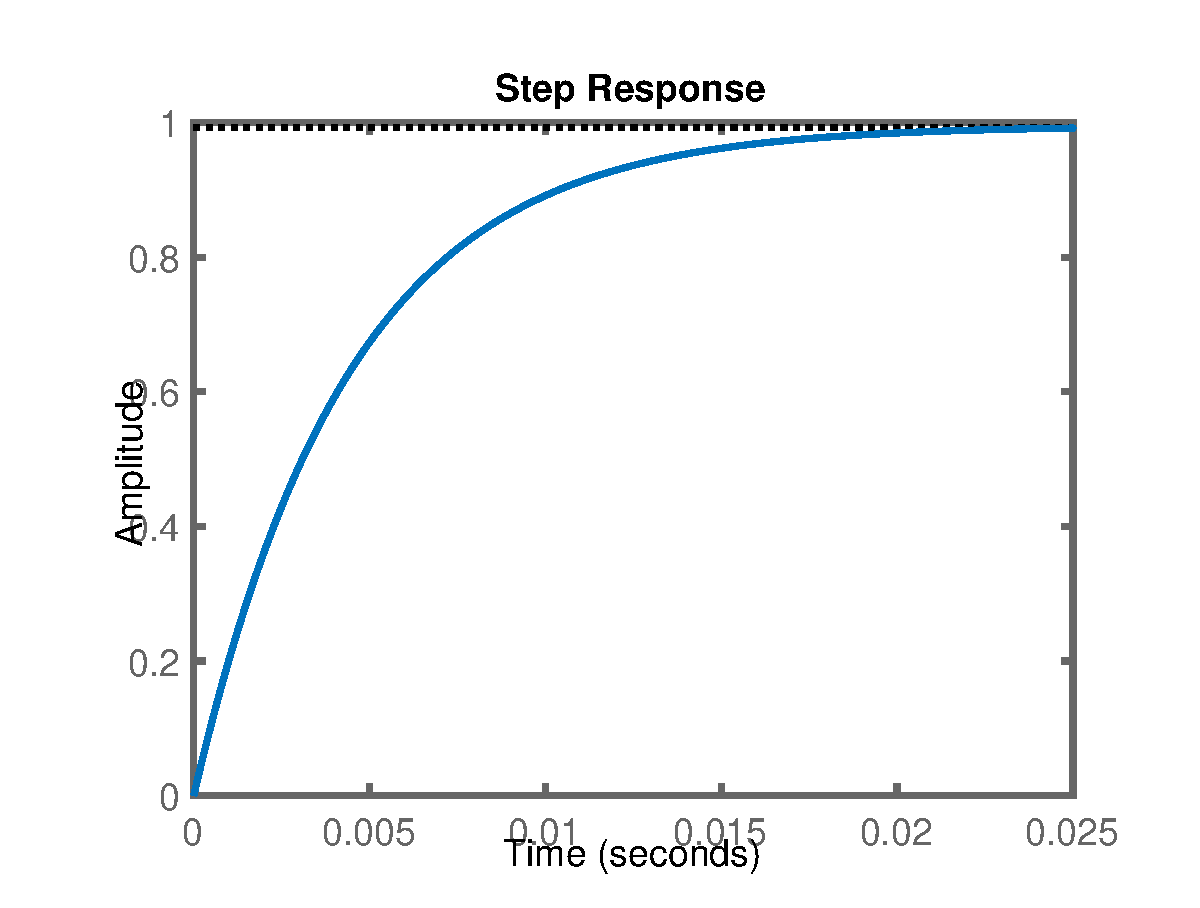
\includegraphics[width=\linewidth]{Bilder/RootLocus_ControlDesign_SysResp_C.eps}
	\caption{Altering root locus by placing a zero in-between two poles}
	\label{Fig_RootLocus_ControlDesign_SysResp_C}
\end{figure}
\newpage
As can be seen from figure \ref{Fig_RootLocus_ControlDesign_SysResp_C}, the design objective for the required control has been achieved for this system. Generally, it is not possible to achieve such a perfect control as in most of the cases the systems are noncanonical and the inputs are more random. Therefore, a different control design using frequency domain anaylsis of the system is emplyoed in all suh cases.

\subsection{General trends of adding a zero or a pole}

In general the following trends from the poles and zero poisitoning in the root locus can be said:
\begin{enumerate}
	\item Adding a zero to the left of poles will makes the system more stable and settle faster.
	\item Adding a zero near the pole or vice-verse will cancel out thier effect (pole-zero cancellation)
	\item Adding a pole will tend to pull the root locus towards right which tends to make the system more unstable and much slower.
\end{enumerate}